\chapter{THỰC NGHIỆM}
\label{Chapter4}

\section{Tập dữ liệu}

\begin{figure}[H]
	\centering
	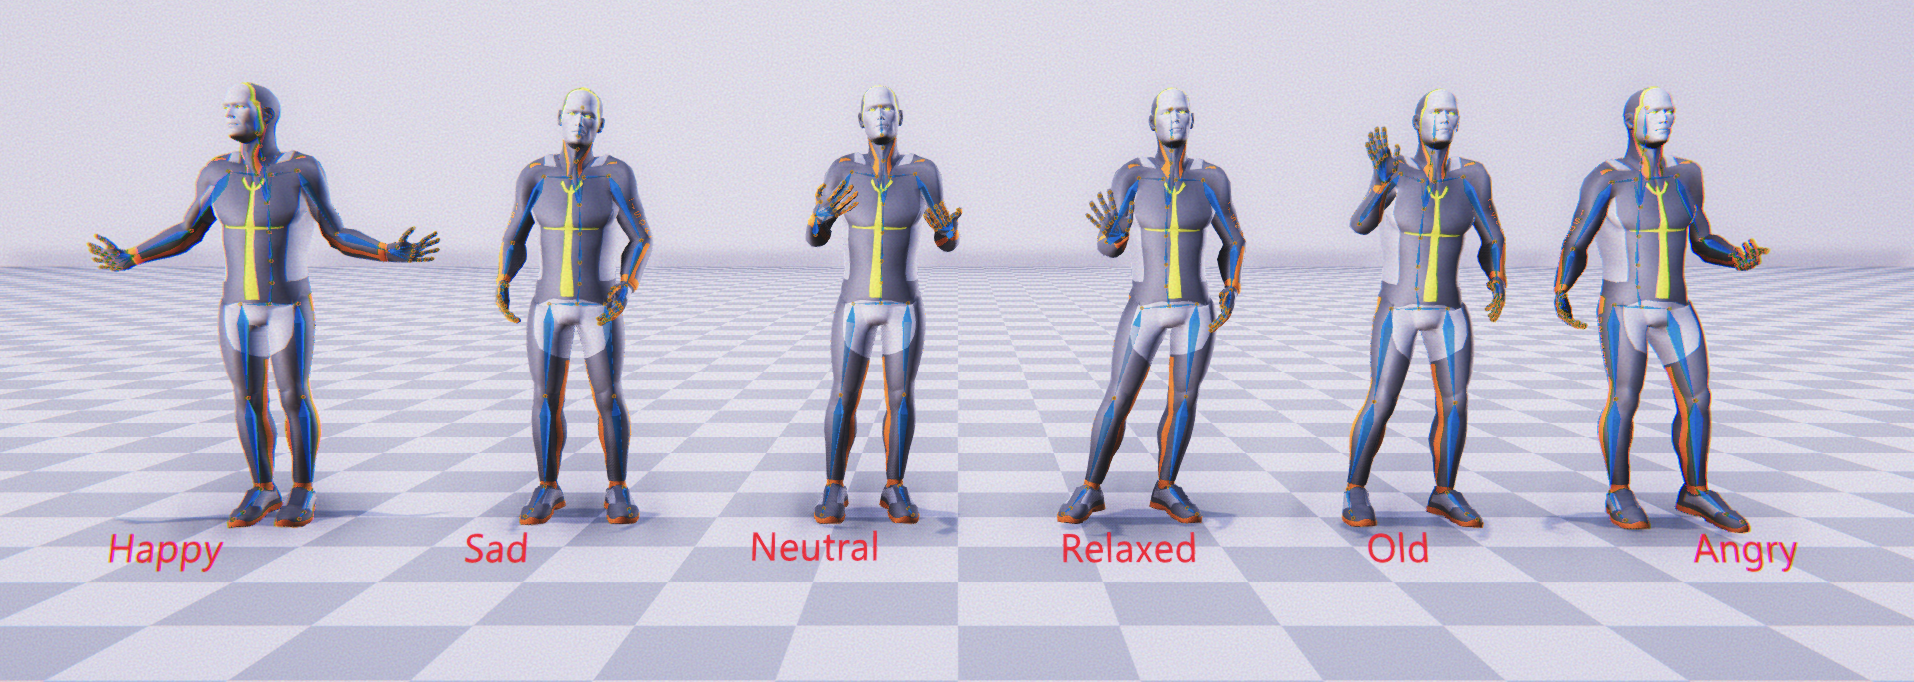
\includegraphics[width=\textwidth]{EmotionAnimation}
	\caption{Minh hoạ về 6 cử chỉ $\texttt{Happy}$, $\texttt{Sad}$, $\texttt{Neutral}$, $\texttt{Old}$, $\texttt{Relaxed}$ và $\texttt{Angry}$}
\end{figure}

Luận văn sử dụng tập dữ liệu ZeroEGGS \cite{ghorbani2022zeroeggszeroshotexamplebasedgesture} là một bộ dữ liệu motion capture được xây dựng để nghiên cứu và phát triển các mô hình tạo cử chỉ. Nó bao gồm 67 đoạn độc thoại do diễn viên motion capture nữ thực hiện, với tổng thời gian là 135 phút. Các đoạn hội thoại trong tập dữ liệu được biểu diễn với 6 cảm xúc khác nhau: $\texttt{Happy}$, $\texttt{Sad}$, $\texttt{Neutral}$, $\texttt{Old}$, $\texttt{Relaxed}$ và $\texttt{Angry}$, giúp mô phỏng nhiều trạng thái cảm xúc khác nhau trong cử chỉ và chuyển động cơ thể. ZeroEGGS cung cấp một nền tảng phong phú để nghiên cứu khả năng kết hợp giữa bài nói và cử chỉ động, phục vụ cho việc tạo ra các mô hình có thể điều chỉnh cử chỉ tương ứng với cảm xúc và ngữ nghĩa của văn bản.

\section{Công đoạn tiền xử lý dữ liệu}
\label{sec:Preprocessing}

Trong công đoạn {1. Tiền xử lý dữ liệu} (\autoref{fig:CommonStage}), các dữ liệu về cử chỉ, giọng nói, văn bản được đọc và xử lý để biểu diễn thành các vector hoặc ma trận thể hiện thông tin về dữ liệu thô.

Đối với \textbf{dữ liệu văn bản}: Luận văn sử dụng thư viện $\texttt{nltk}$ tách các từ, sử dụng $\texttt{contractions}$ để chuyển các từ viết tắt về dạng chuẩn hóa.

Một trong những đóng góp của luận văn là từ dữ liệu giọng nói có sẵn từ tập ZeroEEGS, luận văn đã sử dụng Adobe Speech To Text để chuyển giọng nói thành văn bản, dùng Montreal Forced Aligner \cite{saxon2020robust} của từ điển âm vị Tiếng Anh để căn chỉnh được thời gian tương ứng với số frame của cử chỉ để thu được các TextGrid. Trong TextGrid sẽ có thời gian tương ứng với từng từ, dựa trên thông tin này, luận văn sử dụng  $\texttt{gensim}$ để nhúng vector word2vec.
 

\textbf{Dữ liệu cử chỉ} bao gồm các tệp BVH (BioVision Motion Capture) được thu nhận từ các cảm biến bằng các hệ thống Motion Capture. Trong các tệp BVH, có chứa hai thành phần gồm Hierachy và Motion. Trong đó:

\begin{itemize}
	\item \texttt{HIERARCHY}: là một cây định nghĩa thông tin khung xương bao gồm 75 bone $\{ \mathbf{b}_1, \mathbf{b}_2 \cdots \mathbf{b}_{75} \} $, mỗi bone bao gồm thông tin về vị trí ban đầu (\texttt{OFFSET}), và các loại tham số \texttt{CHANNELS} thể hiện thông tin về loại, thứ tự của góc quay (\texttt{Zrotation}, \texttt{Yrotation} \texttt{Xrotation}) và vị trí (\texttt{Xposition}, \texttt{Yposition}, \texttt{Zposition}) sẽ định nghĩa trong phần \texttt{MOTION}. Bone (thường là \texttt{Hips}) đầu tiên sẽ là bone gốc $\mathbf{b}_{\text{root}}$, là vị trí sau đó sẽ được forward kinematic (động học thuận) để được T-Shape là ví trí ban đầu của toàn bộ khung xương trước khi áp dụng chuyển động.
	
	\item \texttt{MOTION}: là chuỗi các khung hình. Mỗi khung hình là dữ liệu chuyển động thể hiện sự thay đổi của toàn bộ $75$ khung xương đã định nghĩa trong \texttt{CHANNELS} của \texttt{HIERARCHY}.
\end{itemize}


Mô hình của luận văn chuyển dữ liệu từ góc quay Euler sang góc quay Quaternion, với góc quay Quaternion là một véc-tơ gồm 4 phần tử.

\begin{equation} \label{eq:gesturevector}
	\mathbf{g} = \Big[ \mathbf{p}_{\text{root}},  \mathbf{r}_{\text{root}},
	\mathbf{ p }'_{\text{root}},  \mathbf{r}'_{\text{root}},
	\mathbf{p}_{\text{joins}},  \mathbf{r}_{\text{joins}},
	\mathbf{p}'_{\text{joins}},  \mathbf{r}'_{\text{joins}},
	\mathbf{d}_{\text{gaze}}
	\Big]
\end{equation}

Trong  đó với mỗi $\mathbf{g} \in \mathbb{R}^{1141}$ bao gồm:
{
	\begin{itemize}
		\item $\mathbf{p}_{\text{root}} \in \mathbb{R}^3$: tọa độ của điểm gốc
		\item $\mathbf{r}_{\text{root}} \in \mathbb{R}^4$: Góc quay của điểm gốc
		\item $\mathbf{p}'_{\text{root}} \in \mathbb{R}^3$: Vận tốc thay đổi của tọa độ gốc
		\item $\mathbf{r}'_{\text{root}} \in \mathbb{R}^3$: Vận tốc thay đổi của góc quay gốc
		
		\item $\mathbf{p}_{\text{joins}} \in \mathbb{R}^{3 n_{\text{join} }}$: tọa độ của các khung xương
		\item $\mathbf{r}_{\text{joins}} \in \mathbb{R}^{6 n_{\text{join} }}$: Góc quay của các khung xương theo mặt phẳng X và Y
		\item $\mathbf{p}'_{\text{joins}} \in \mathbb{R}^{3n_{\text{join} }}$: Vận tốc thay đổi của tọa độ các khung xương
		\item $\mathbf{r}'_{\text{joins}} \in \mathbb{R}^{3n_{\text{join} }}$: Vận tốc thay đổi của góc quay các khung xương
		\item $\mathbf{d}_{\text{gaze}} \in \mathbb{R}^3$: Là hướng nhìn
\end{itemize}}

Chuỗi cử chỉ ban đầu có dữ liệu là góc quay sẽ được chuyển thành các góc quay radian, từ góc quay radian ở dạng Euler sẽ được chuyển sang góc quay Quaternion, với quá trình cụ thể được trình bày trong \autoref{appendix:BVHData:QuaternionConvert}.

\textbf{Dữ liệu giọng nói}: $\mathbf{a}_{\text{raw}} \in \mathbb{R}^{ \text{length } }$ là chuỗi giọng nói thô được đọc ở sample rate 16000, sau đó được cắt thành $\mathbf{a} \in \mathbb{R}^{64000}$ tương ứng với 4 giây. Luận văn sử dụng thư viện \texttt{ffmpeg-normalize} để chuẩn hóa tiếng nói nhỏ hơn so với giọng nói gốc.

\textbf{Cảm xúc}: Dữ liệu cảm xúc sẽ được biểu diễn bằng một vector one-hot encoding sẵn. Trong quá trình lấy mẫu, tên tệp sẽ định nghĩa luôn thông tin về cảm xúc mong muốn.

Toàn bộ dữ liệu sẽ được lưu bằng $\texttt{h5}$ được dùng để lưu trữ dữ liệu.

\section{Quá trình huấn luyện}

Toàn bộ quá trình huấn luyện mô hình được thực hiện trong vòng 1 ngày với các tham số sau: số bước huấn luyện $T = 1000$, sử dụng GPU Nvidia 3090, và chia tập dữ liệu theo tỷ lệ $8:1:1$ cho các tập training, testing và validation. Learning rate được thiết lập là $3 \times 10^{-5}$, với batch size là $640$ và tổng cộng $43,853$ mẫu. 
$\gamma = 0.1$.

$\beta$ bắt đầu từ $0.5 \rightarrow 0.999$

Quá trình huấn luyện được triển khai trên mã nguồn công khai tại: \hyperlink{https://github.com/hmthanh/OHGesture}{Github/OHGesture} \footnote{\url{https://github.com/hmthanh/OHGesture}}.


\section{Quá trình sử dụng Unity để kết xuất}
\label{sec:Render}

Để trực quan hóa quá trình sinh cử chỉ từ dữ liệu đầu ra của mô hình, trong công đoạn \textit{7. Kết xuất} (\autoref{fig:CommonStage}) luận văn sử dụng Unity, kết thừa mã nguồn từ mô hình DeepPhase \cite{starke2022deepphase}  . Dữ liệu sau khi sinh là tệp BVH (BioVision Motion Capture). Trong Unity, luận văn bổ sung mã nguồn C-Sharp để kết xuất theo vị trí tọa độ và nhãn tương ứng, với vị trí và góc quay của các xương được biểu diễn dưới dạng quaternion.

Chi tiết phần render cử chỉ được sinh ra, tôi trình bày ở \autoref{Appendix3}.

Mã nguồn chương trình Unity được luận văn công khai ở \hyperlink{https://github.com/DeepGesture/deepgesture-unity}{Github/DeepGesture-Unity}
\footnote{\url{https://github.com/DeepGesture/deepgesture-unity}}.
